\documentclass[]{beamer}
\mode<presentation>
{
  \usetheme{Warsaw}
  \definecolor{mcgarnet}{rgb}{0.38, 0, 0.08}
  \definecolor{mcgray}{rgb}{0.6, 0.6, 0.6}
  \setbeamercolor{structure}{fg=mcgarnet,bg=mcgray}
  %\setbeamercovered{transparent}
}


\usepackage[english]{babel}
\usepackage[latin1]{inputenc}
\usepackage{times}
\usepackage[T1]{fontenc}
\usepackage{tikz}
\usepackage{graphicx}
\usepackage{fancyvrb}
\usepackage{adjustbox}

\newcommand{\imagesource}[1]{{\centering\hfill\break\hbox{\scriptsize Image Source:\thinspace{\small\itshape #1}}\par}}

\title{08 - Going Loopy - Part 1}


\author{Dr. Robert Lowe\\}

\institute[Maryville College] % (optional, but mostly needed)
{
  Division of Mathematics and Computer Science\\
  Maryville College
}

\date[]{}
\subject{}

\pgfdeclareimage[height=0.5cm]{university-logo}{images/Maryville-College}
\logo{\pgfuseimage{university-logo}}



\AtBeginSection[]
{
  \begin{frame}<beamer>{Outline}
    \tableofcontents[currentsection]
  \end{frame}
}


\begin{document}

\begin{frame}
  \titlepage
\end{frame}

\begin{frame}{Outline}
  \tableofcontents
\end{frame}


% Structuring a talk is a difficult task and the following structure
% may not be suitable. Here are some rules that apply for this
% solution: 

% - Exactly two or three sections (other than the summary).
% - At *most* three subsections per section.
% - Talk about 30s to 2min per frame. So there should be between about
%   15 and 30 frames, all told.

% - A conference audience is likely to know very little of what you
%   are going to talk about. So *simplify*!
% - In a 20min talk, getting the main ideas across is hard
%   enough. Leave out details, even if it means being less precise than
%   you think necessary.
% - If you omit details that are vital to the proof/implementation,
%   just say so once. Everybody will be happy with that.

\section{Precondition and Postcondition Loops}
\begin{frame}[fragile]{The Precondition Loop}
  \begin{columns}
    \column{0.5\textwidth}

    \begin{block}{While Loop Syntax}
      \verb!while(! \textit{condition} \verb!)! 
      \newline\verb!    ! \textit{statement/block}
    \end{block}
    
    \vspace{0.5cm}

    \begin{itemize}[<+(1)->]
        \item The \texttt{while} loop is called a precondition loop.
        \item The condition is checked before the loop body is
            executed.
        \item The loop body is executed zero or more times.
    \end{itemize}

    \column{0.5\textwidth}
    \begin{center}
      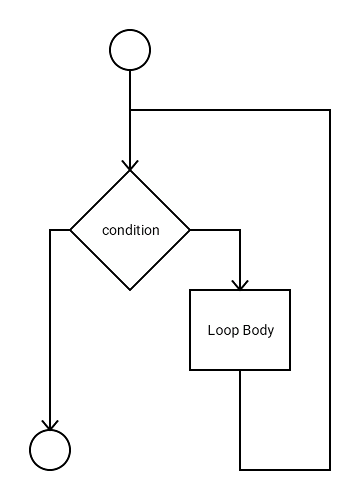
\includegraphics[width=0.8\textwidth]{images/while}
    \end{center}
  \end{columns}
\end{frame}

\begin{frame}[fragile]{The Postcondition Loop}
  \begin{columns}
    \column{0.5\textwidth}

    \begin{block}{While Loop Syntax}
      \verb!do! 
      \newline\verb!    ! \textit{statement/block}
      \newline\verb!while(! \textit{condition} \verb!);! 
    \end{block}
    
    \vspace{0.3cm}

    \begin{itemize}[<+(1)->]
        \item The \texttt{do..while} loop is called the postcondition
        loop.
        \item The condition is checked after the loop body.
        \item Executes 1 or more times.
        \item Commonly used with input validation and menus.
    \end{itemize}

    \column{0.5\textwidth}
    \begin{center}
      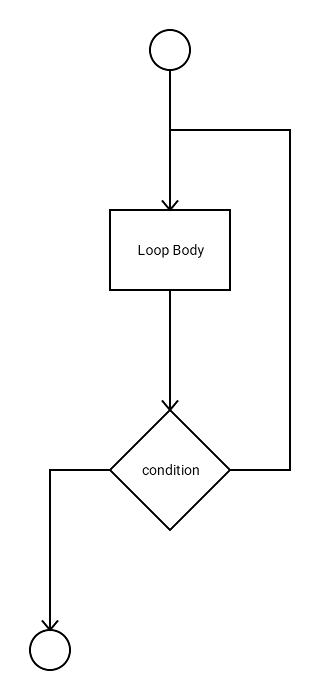
\includegraphics[height=0.9\textheight]{images/do-while}
    \end{center}
  \end{columns}
\end{frame}

\begin{frame}[fragile]{Example: \texttt{examples/08-Loopy/validate.cpp}}
    \begin{adjustbox}{max totalheight=0.8\textheight, max width=0.9\textwidth}
        \begin{BVerbatim}
    int x;       //the number to be validated.
    bool valid;  //whether the choice is valid

    //get a valid choice
    cout << "Enter a number between 1 and 5." << endl;
    do {
        //get a number
        cout << "number: ";
        cin >> x;

        //check validity
        valid = x>=1 and x<=5;

        //report errors
        if(not valid) {
            cout << "Invalid selection.  Please try again." << endl;
        }
    } while(not valid);

    cout << "Thank You" << endl;
        \end{BVerbatim}
    \end{adjustbox}
\end{frame}

\begin{frame}[fragile]{Example: \texttt{examples/08-Loopy/menu.cpp}}
    \begin{adjustbox}{max totalheight=0.8\textheight, max width=0.9\textwidth}
        \begin{BVerbatim}
    int choice;

    //Run the menu
    do {
        cout << "1.) Option One" << endl
             << "2.) Option Two"<< endl
             << "3.) Exit" << endl
             << "Choice? ";
        cin >> choice;

        //do the selection
        if(choice == 1) {
            cout << "Option One" << endl;
        } else if(choice == 2) {
            cout << "Option Two" << endl;
        } else if(choice != 3) {
            cout << "Invalid selection, please try again." << endl;
        }
    } while(choice != 3);
        \end{BVerbatim}
    \end{adjustbox}
\end{frame}


\begin{frame}[fragile]{Enumerated Types}
    \begin{itemize}[<+->]
        \item An enumerated type or \texttt{enum} specifies a type
            with a fixed set of numeric values.
        \item \verb!enum menu_choices {ONE=1, TWO, EXIT};!
        \item We get three constants, \texttt{ONE}, \texttt{TWO},
            \texttt{EXIT} who's values are 1, 2, and 3.
        \item Often used with menus to label their selections with
            named constants in the code.
    \end{itemize}
\end{frame}


\begin{frame}[fragile]{Example: \texttt{examples/08-Loopy/menu2.cpp}}
    \begin{adjustbox}{max totalheight=0.8\textheight, max width=0.9\textwidth}
        \begin{BVerbatim}
    enum menu_choice { ONE=1, TWO, EXIT };
    int choice;

    //Run the menu
    do {
        cout << "1.) Option One" << endl
             << "2.) Option Two"<< endl
             << "3.) Exit" << endl
             << "Choice? ";
        cin >> choice;

        //do the selection
        if(choice == ONE) {
            cout << "Option One" << endl;
        } else if(choice == TWO) {
            cout << "Option Two" << endl;
        } else if(choice != EXIT) {
            cout << "Invalid selection, please try again." << endl;
        }
    } while(choice != EXIT);
        \end{BVerbatim}
    \end{adjustbox}
\end{frame}


\section{Exercises}
\begin{frame}{Challenge \texttt{labs/week5/guess.cpp}}
    We will write a guessing game!
    \begin{itemize}[<+->]
        \item The computer will generate a random integer between
            1 and 100.
        \item The computer will ask us to guess the number.
        \item If we guess a number that is too low, the computer will
            tell us it is too low.
        \item If we guess a number that is too high, the computer will
            let us know if it is too high.
        \item We continue guessing until we guess the number.
        \item After we guess correctly, the computer will tell us how
            many tries it took us.
    \end{itemize}
\end{frame}


\begin{frame}{Challenge: \texttt{labs/week5/stock.cpp}}
    \begin{itemize}[<+->]
        \item Copy your most recent \texttt{stock.cpp} into your week5
            directory.
        \item Add an enumerated type for the menu selections.
        \item Rework your menu so it is in a loop.  It should allow
            you to keep using the system until you choose the option
            that causes it to exit.
    \end{itemize}
\end{frame}


\begin{frame}{Week 5 Lab Requirements}
    You must have the following programs completed for full credit in
    week5.
    \begin{enumerate}
        \item \texttt{multiply.cpp}
        \item \texttt{guess.cpp}
        \item \texttt{stock.cpp} (with enum and menu loops).
    \end{enumerate}
\end{frame}


\end{document}


